% -----------------------------------------------------------------------------
% UFRJ
% PPGI
% MAB 733 Sistemas Distribuídos
%
% Revisado em 23/04/2013
% Autor: Cristiano Gurgel de Castro
% -----------------------------------------------------------------------------

\chapter{Desenvolvimento e Arquitetura}

Houve algumas tentativas de desenvolvimento da aplicação até conseguirmos a
comunicação com os diferentes tipos de serviços web. Iremos apresentar parte dos
problemas encontrados. Nas próximas seções são apresentadas as tentativas de
implementação do serviço até conseguirmos implementá-lo. São mostrados partes de
código, a arquitetura códigos e uma descrição de boa parte dos problemas
encontrados. 

\section{Desenvolvimento na IDE \NetBeansv}

O programa é composto por uma aplicação \desktop\ cliente \Java\footnote{Versão
\Javav} de nome \code{CalculatorGui}. Essa aplicação simples trata-se de uma
calculadora que efetua algumas operações básicas. 

Primeiramente foi desenvolvido um serviço web em Java para a implementação das 4
operações básicas. No projeto cliente, foi criada uma fachada para essa camada
de negócios: \code{IMathOperations} e duas implementações desta fachada:
\code{MathOperations}, que é local, e \code{RemoteMathOperations}, a qual
se utiliza dos serviços de um \proxy\ para um serviço externo. A arquitetura então
desenvolvida é representada na Fig.  \ref{fig:arquitetura:calc}. Um trecho do
código da classe \code{RemoteMathOperations} com a chamada ao método de soma do
serviço Web é mostrado no Código \ref{cod:add}\footnote{Os trechos de código são
mostrados no apêndice \ref{sec:codigos}}.

\begin{figure}[htb]
  \centering
    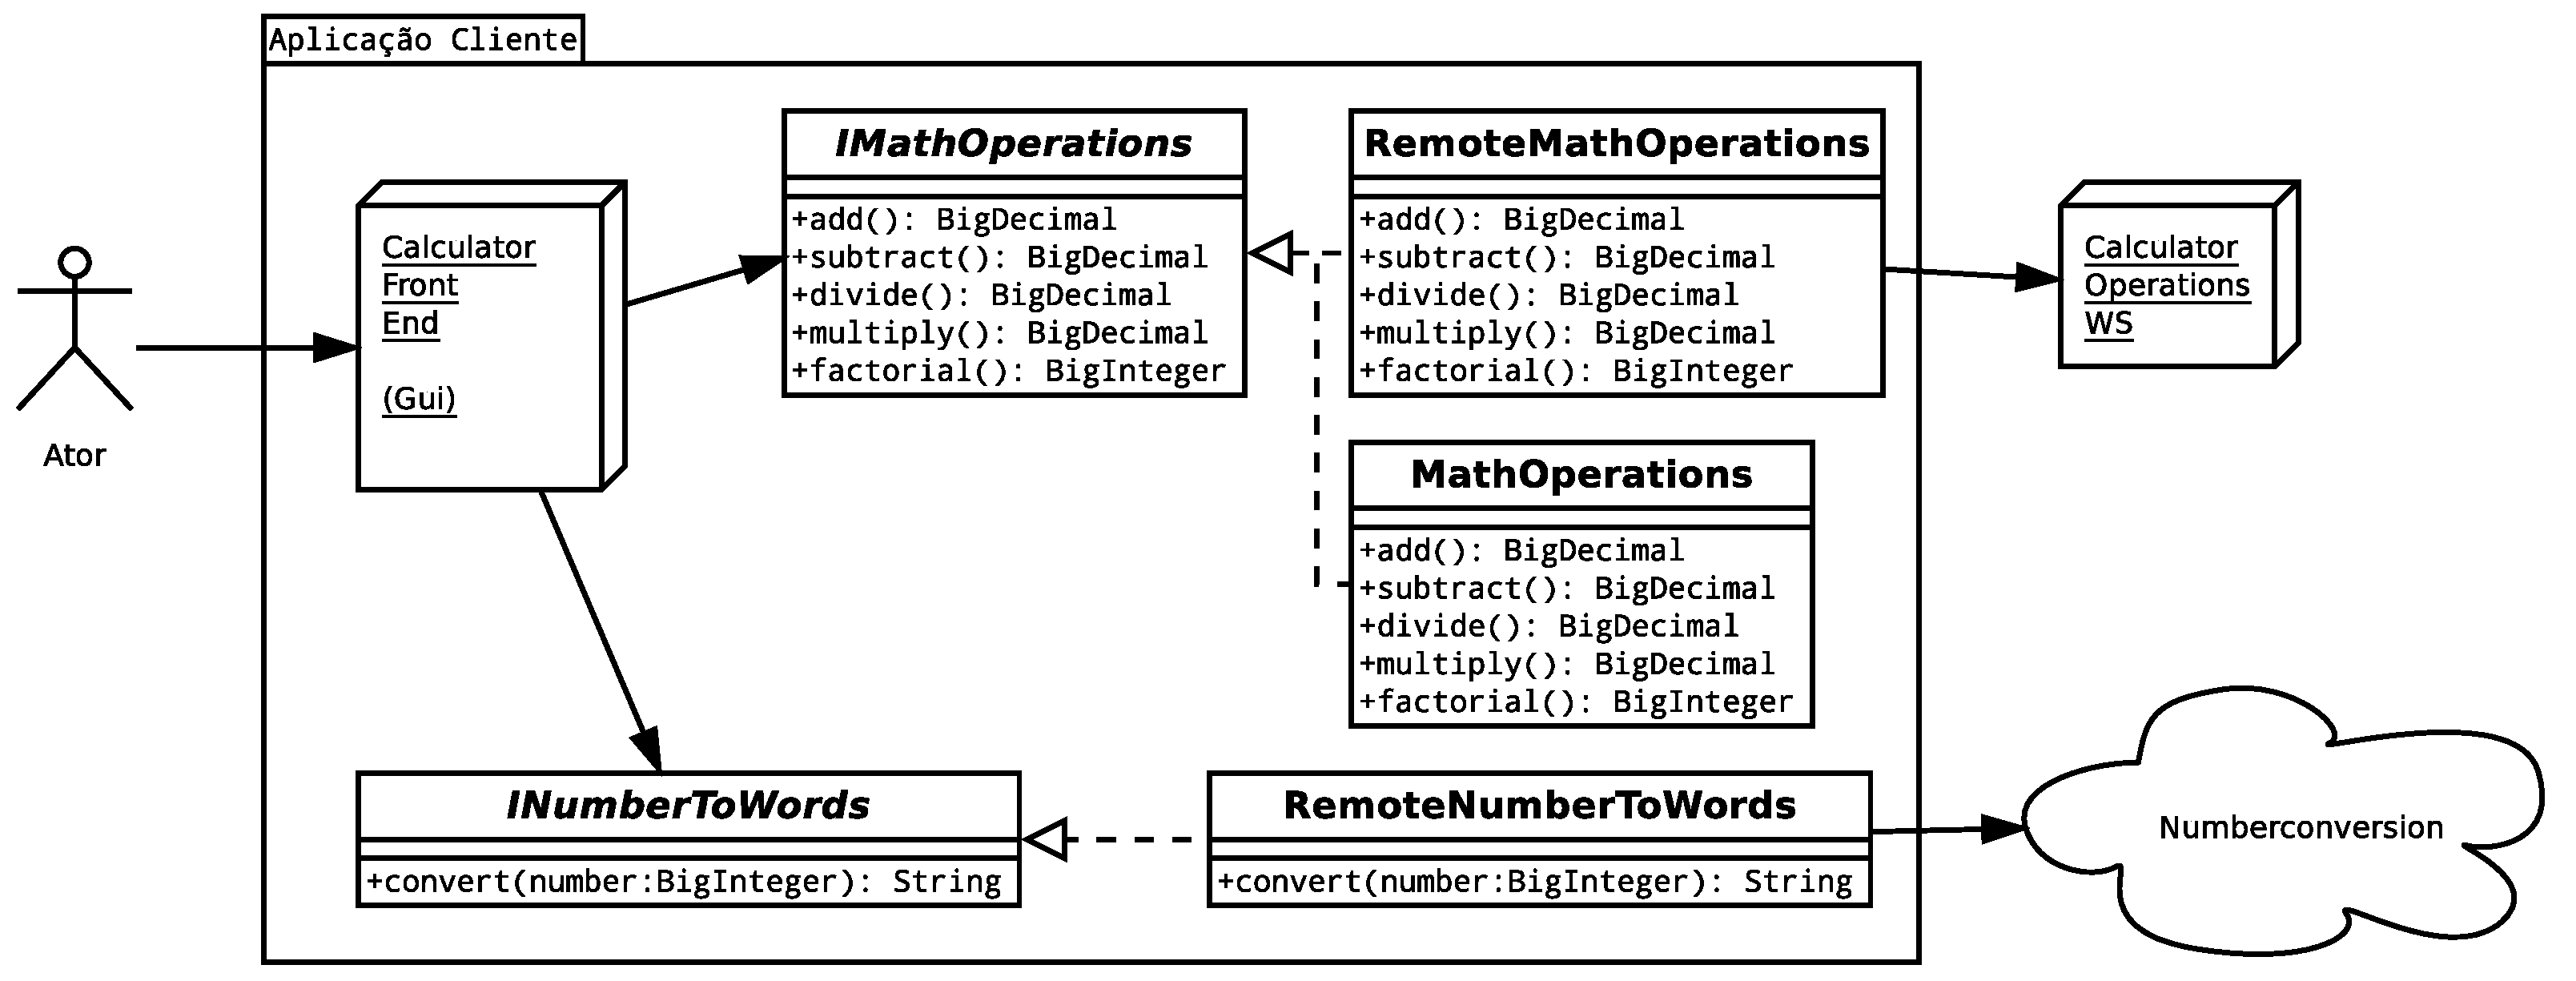
\includegraphics[width=\textwidth]{imgs/calculadora}
  \caption{Arquitetura da aplicação cliente.}
  \label{fig:arquitetura:calc}
\end{figure}

O serviço \code{CalculatorWebService} provê uma implementação das quatro
operações básicas. O \WebService\ foi criado
utilizando o IDE \NetBeansv\ juntamente com servidor de aplicação \Glassfish, o
qual já vem integrado à IDE e no qual foi hospedado o serviço. O \NetBeans\
provê uma funcionalidade muito prática de criação de \WebService s, através da
utilização da opção \textbf{Serviço Web} do Assistente de criação de projetos, o
qual automaticamente cria uma classe com a implementação do Serviço Web. O
usuário pode visualizar uma tela chamada \emph{Projeto} contendo uma
visualização amigável das operações efetuadas a serem implementadas no serviço
(ver Figura \ref{fig:arquitetura:design}). Através dessa tela, foram
configuradas as quatro operações que o \WebService\ deve fornecer: as quatro
operações básicas. Cada uma dessas operações recebem dois \code{float}s como
parâmetros e retornam um \code{float} como resultado.  Após a configuração das
operações, a tarefa seguinte foi inserir o código de implementação. Um trecho de
código exemplo, com a operação de adição do \WebService, é mostrado no código
\ref{cod:calculatorws}:

\begin{figure}[htb]
  \centering
  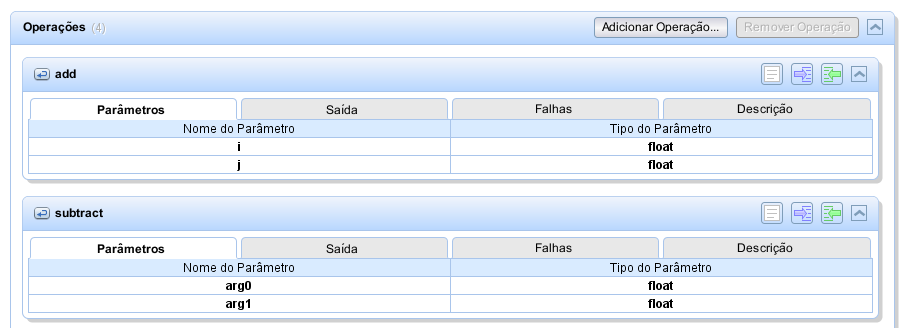
\includegraphics[width=\textwidth]{imgs/webservice-design}
  \caption{Tela de design de um \WebService}
  \label{fig:arquitetura:design}
\end{figure}

O serviço disponível publicamente utilizado foi o \emph{Number Conversion}
encontrado a partir do site \url{xmethods.net}. Segundo sua
descrição\footnote{Descrição encontrada em
\url{http://www.dataaccess.com/webservicesserver/numberconversion.wso}} ele
possui dois métodos: o primeiro (\code{NumberToWords}) contém um serviço de
escrita de número por extenso na língua inglesa, recebendo como parâmetro um
{inteiro}; o segundo (\code{NumberToDollars}) contém uma fun\-cio\-na\-li\-da\-de
semelhante para conversão para valores monetários em dólar. Para o presente
trabalho foi utilizado apenas o primeiro método: \code{NumberToWords}.

Para o acesso ao serviço Web foi utilizada uma facilidade do \NetBeans\ na
aplicação cliente da calculadora: a criação de um ``Cliente para serviço Web''.
Esse componente da IDE foi adicionada ao projeto cliente de calculadora, e
através de um Assistente para a configuração. Um dos parâmetros informados foi a
URL do WSDL do serviço\footnote{a saber
\url{http://www.dataaccess.com/webservicesserver/numberconversion.wso?WSDL}}. Uma
funcionalidade \textbf{SAY} foi então adicionada ao cliente para a chamada ao
serviço, através de uma fachada \code{INumberToWords}. Uma
classe \code{NumberToWords} foi criada para a executar a chamada ao
\proxy\ do \WebService. Essa chamada ao serviço web externo é mostrado no código
\ref{cod:numberconv}.

No entanto um erro de transporte mostrado no código \ref{cod:httperror}, foi
lançado durante a chamada de serviço. Interessante notar que um outro projeto
cliente Java foi criado para testar a comunicação com o serviço Web
\estrangeiro{Number Conversion} e a comunicação ocorreu sem maiores problemas.
Para um segundo teste de acesso ao serviço, Um outro cliente, dessa vez escrito
na linguagem \php\, também executou normalmente o acesso ao serviço. O Código
\ref{cod:phpclient} mostra o acesso ao serviço externo com um cliente \php. Para
então contornar o problema com o cliente, o código fonte do projeto Calculadora
original, foi exportado e importado no projeto cliente o qual conseguiu acesso
ao \WebService\ e assim foi executada a chamada ao método \code{NumberToWords}.

Finalmente, passamos a implementação de um serviço em outra linguagem de
programação para utilização na calculadora. Primeiramente foi testado a
comunicação com um serviço \estrangeiro{Hello World} simples. Foi escolhida a
linguagem de programação \PHP\ para a criação de um outro serviço local, o
código do aplicação \estrangeiro{Hello World} é apresentado no Código
\ref{cod:phphello}. Utilizou-se a biblioteca \NuSOAPv\ do \PHP\ para a criação do
serviço web e geração automática do WSDL. No entanto ao tentar-se criar o
cliente do \WebService para utilização no projeto Calculadora utilizando-se o
assistente do \NetBeans\ nos deparamos com um problema que não conseguimos
contornar: não se conseguiu gerar o \estrangeiro{proxy} . Primeiramente, o
assistente de criação de \proxy\ gerou uma mensagem de erro na criação do
\WebService\ a partir do WSDL gerado pela biblioteca \NuSOAP\ informando um
erro de impossibilidade de criação devido ao Estilo RPC. Foi tentado então
modificar o estilo do WSDL gerado pelo \NuSOAP\ de ``RPC'' para ``Document''. O
\NetBeans\ conseguiu então gerar as classes \proxy\ para a utilização do
serviço, porém ao utilizar o serviço, deparamos com a seguinte mensagem de
exceção: \code{Couldn't create SOAP message due to exception: unexpected XML
tag}. Para contornar esse problema, foi utilizada a IDE \Eclipsev.

% TODO colocar um recorte do erro gerado ao tentarmos criar um proxy NetBeans

\section{Desenvolvimento na IDE \Eclipsev}

Passamos a utilizar o \Eclipsev\ para tentar a comunicação com o serviço gerado
pelo código \PHP. Foram utilizados, integrados ao \Eclipse, o \ApacheTomcatv\ e o
\ApacheAxisDoisv. Primeiramente para os testes de aplicação, foi seguido o
tutorial de criação de um servidor e cliente através da utilização do
\ApacheAxisDoisv\footnote{\url{http://www.eclipse.org/webtools/community/tutorials/BottomUpAxis2WebService/bu_tutorial.html}}.
Primeiramente ao tentarmos criar um \textbf{Dynamic Web Project} tínhamos nos
deparado com o seguinte erro: \code{The Apache Axis2 Web service runtime in
Tomcat v7.0 Server does not support the service project ConverterProj.}. Ao
seguir o tutorial porém foi esclarecido que o erro era causado por não ter-se
habilitado o \estrangeiro{facet} \code{Axis2 Web Services} para o projeto o qual
gostaríamos de adicionar um serviço web.

O próximo passo foi desenvolver um cliente simples de teste de forma a consumir três
serviços: o serviço Java local gerado a partir do Tutorial apresentado no parágrafo
anterior (\code{Converter}), o serviço provido na web (\estrangeiro{Number Conversion})
e o serviço provido pelo servidor Apache local escrito em \php. As
classes \estrangeiro{stub} para o acesso ao cliente foram criados através do
assistente \textbf{Web Service Client}. O código desse cliente de teste para
utilizar os serviços Web a partir dos \stub s gerados é mostrado no trecho de
código \ref{cod:javaeclipseclient}

Com a execução correta desse código partiu-se para a importação dos projetos
desenvolvidos anteriormente em \NetBeans\ para a plataforma \Eclipse. E assim
pudemos desenvolver a calculadora para utilizar também os serviços de um
\WebService\ local escrito em \PHP. O serviço escrito em PHP foi apenas uma
operação de fatorial que recebe e retorna um parâmetro do tipo \code{xsd:int}
A arquitetura final da aplicação é mostrada
na Fig. \ref{fig:arquitetura:final} 

\begin{figure}[htb]
  \centering
  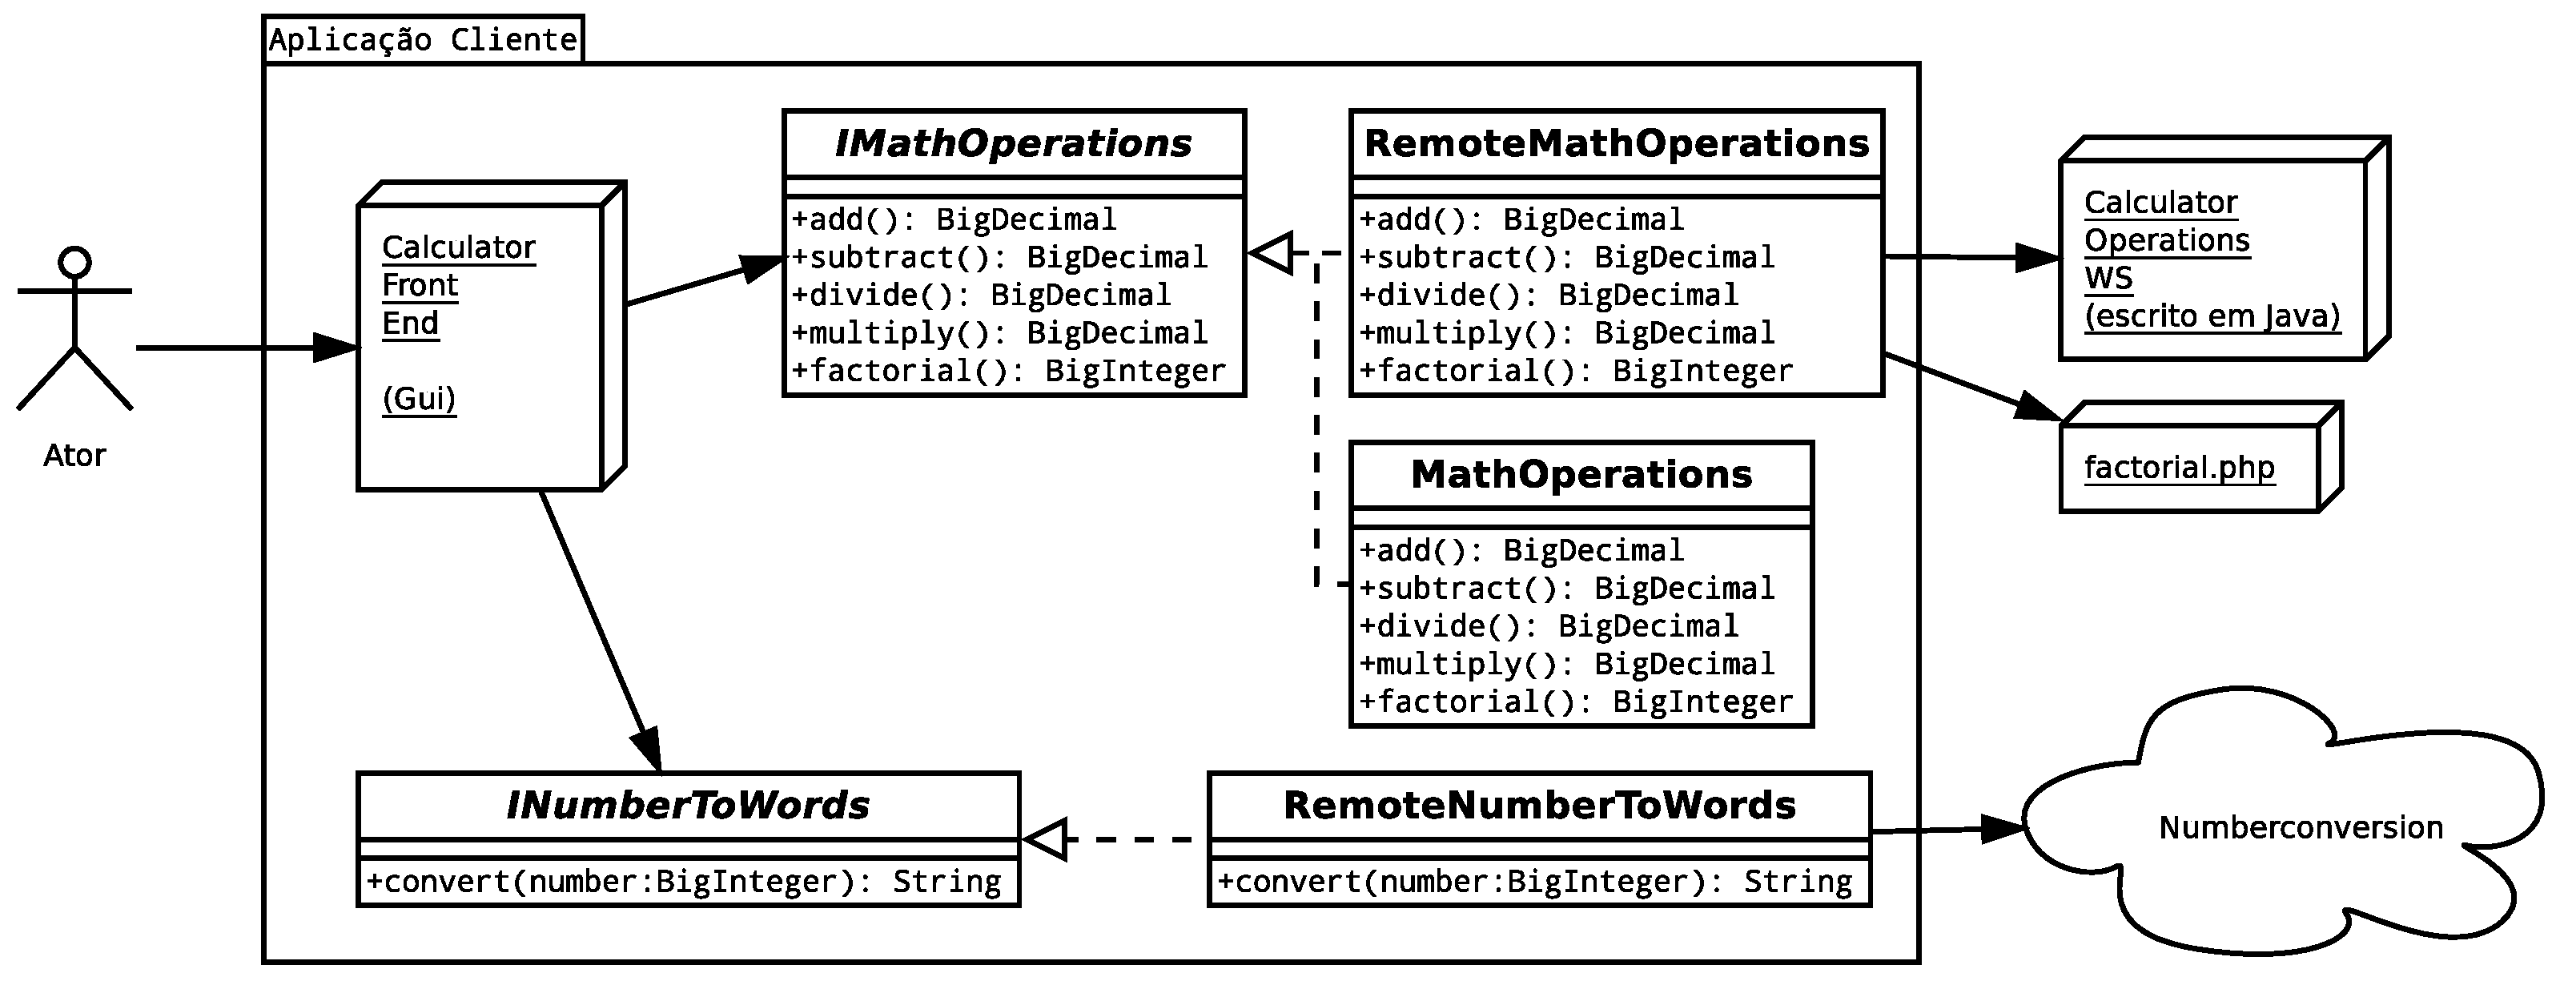
\includegraphics[width=\textwidth]{imgs/arquitetura_final}
  \caption{Arquitetura final da aplicação Calculadora escrita em Java.}
  \label{fig:arquitetura:final}
\end{figure}

Um trecho de código do serviço PHP utilizado para a implantação do servidor de
cálculo do fatorial de um número é mostrado no Código \ref{cod:phpfactorial}. Os
trechos de código que requisitam os serviços web utilizados são mostrados nos
códigos \ref{cod:remote:math:eclipse} e \ref{cod:remote:conversion:eclipse}. A
tela principal da aplicação calculadora é mostrada na Fig.
\ref{fig:arquitetura:gui}. 

\begin{figure}[htb]
  \centering
  \includegraphics[]{imgs/screenshot}
  \caption{Interface gráfica do cliente Calculadora.}
  \label{fig:arquitetura:gui}
\end{figure}
